\newpage
\section{实数基本定理}
这六个定理虽然出发的角度不同,但是都是描述实数连续性这同一回事,他们之间是相互等价的,
即任取其中两个定理,他们可以相互证明。他们在证明过程中相互联系。对同一个定理的证明,
虽然不同的定理作为工具会使证明有简繁之分,有的用的是类似的证明方法,有的出发点与站的角度不同,
但最后却能殊途同归。而有时使用同一个定理,也可能有不同的方法。即是方法相同,也有可能有不同的细节。
作为工具,他们又各具特点。而这些都是值得我们去注意与发现的!   

\vspace*{1em}
\begin{theorem}[实数基本定理]
    \noindent\ding{172} 确界存在定理:非空有上 (下)界数集,必有上 (下)确界。%英文字符和中文字符之间加一个空格不会警告

    \noindent\ding{173} 单调有界收敛原理:任何单调有界数列必有极限。

    \noindent\ding{174} 区间套定理:若$\{\left [ a_n,b_n \right ]\}$是一个区间套,则存在唯一一点$\xi$,使得$\xi\in \left [ a_n,b_n \right ] ,n=1,2,\cdots $

    \noindent\ding{175} \textit{Heine-Borel}有限覆盖定理:设$\left [ a,b \right ]$是一个闭区间,H为$\left [ a,b \right ]$的一个开覆盖,则在H中
    存在有限个开区间,它构成$\left [ a,b \right ]$上的一个覆盖。

    \noindent\ding{176} \textit{Weierstrass}聚点定理 (\textit{Bolzano}致密性定理:有界无穷数列必有收敛子列):直线上的有解无限点集至少有一个聚点。

    \noindent\ding{177} \textit{Cauchy}收敛准则:数列$\{a_n\}$收敛 $\Longleftrightarrow$对任给定的正数$\varepsilon$,总存在某一个自然数$N$,使得$\forall m,n>N$时,
    都有$\left| a_m-a_n \right| < \varepsilon\Longleftrightarrow \{a_n\}$ 是基本数列。
\end{theorem}

\begin{proof}
如图所示
\begin{center}
    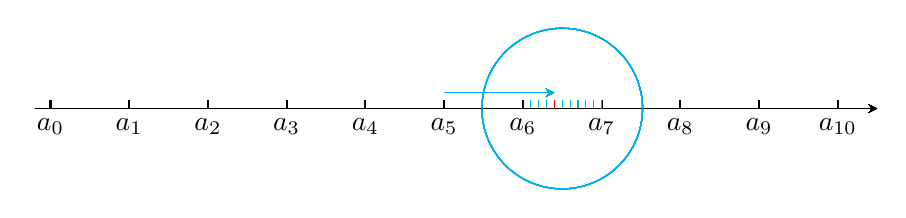
\begin{tikzpicture}[>=stealth]
        \foreach \i in {0, 1, ..., 10}
        {
            \draw[ ->] (-0.2, 0)--(10.5, 0);
            \draw[cyan] (6+\i/10, 0)--(6+\i/10, 3pt);
            \draw[red] (6.4, 0)--(6.4, 3pt);
            \draw[thick] (\i, 0)node[below]{$a_{\i}$}--(\i, 3pt);
            \draw[cyan] (6.5, 0) circle [radius=1.02];
            \draw[->, cyan] (5, 0.2) -- (6.4, 0.2);
        }
    \end{tikzpicture}
\end{center}
\end{proof}

\clearpage